\documentclass{beamer}
\mode<presentation>
\usetheme{Diku} % was: Warsaw
\beamertemplatenavigationsymbolsempty
%\setbeamercovered{transparent}
\usepackage{graphicx}
\usepackage{color}
\usepackage{verbatim}
\usepackage{cmap,enumerate}
\usepackage[utf8x]{inputenc}
%\usepackage[T1]{fontenc}
\usepackage[danish]{babel}
\pagestyle{empty}
\setlength{\unitlength}{1cm}

\title{Mere om rekursive typer}

\date[2016]{PoP 14102016}

\author{Torben Ægidius Mogensen}

\begin{document}

\usebackgroundtemplate{
  \includegraphics[width=\paperwidth,height=\paperheight]{Forside}
}
\begin{frame}
\titlepage
\end{frame}


\usebackgroundtemplate{
  \includegraphics[width=\paperwidth,height=\paperheight]{Baggrund}
}

%%

\definecolor{darkgreen}{rgb}{0,0.4,0}

\definecolor{darkred}{rgb}{0.5,0,0}

\begin{frame}[fragile=singleslide]
\frametitle{Lister som rekursive typer}

Listetypen \texttt{'a list} er også en rekursiv type:

\begin{verbatim}
type 'a list = [] | 'a :: 'a list
\end{verbatim}

Ovenstående kan ikke skrives i F\#, da konstruktornavne skal starte med stort
bogstav, og infix konstruktorer er ikke tilladt.  Men man kan uden
videre skrive en ækvivalent definition:

\begin{verbatim}
type 'a liste = Nil | Cons of 'a * 'a liste
\end{verbatim}

hvor \texttt{Nil} svarer til \texttt{[]}, og \texttt{Cons} svarer til
en præfixudgave af \texttt{::}.


\end{frame}

\begin{frame}[fragile=singleslide]
\frametitle{Funktioner på vores egen listetype}

Vi kan sammenligne funktionsdefinitioner på \texttt{'a list} med
funktionsdefinitioner på \texttt{'a liste}:

\renewcommand{\baselinestretch}{0.85}
{\small
\begin{verbatim}
let rec listLength (xs : 'a list) =
  match xs with
  | [] -> 0
  | x :: xs -> 1 + listLength xs

let rec listeLength (xs : 'a liste) =
  match xs with
  | Nil -> 0
  | Cons (x, xs) -> 1 + listeLength xs

let rec listMap f (xs : 'a list) =
  match xs with
  | [] -> []
  | x :: xs -> (f x) :: listMap f xs

let rec listeMap f (xs : 'a liste) =
  match xs with
  | Nil -> Nil
  | Cons (x, xs) -> Cons (f x, listeMap f xs)
\end{verbatim}
}


\end{frame}

\begin{frame}[fragile=singleslide]
\frametitle{Sammenligning af opremsede typer}

Hvis vi har typen:

\begin{verbatim}
type day = Mon | Tue | Wed | Thu | Fri | Sat | Sun
\end{verbatim}

kan man sammenligne værdierne med \texttt{=}, \texttt{<}, osv:

\vspace{2ex}

\texttt{
\begin{tabular}{lcl}
Mon = Mon & $\leadsto$ & true \\
Mon = Tue & $\leadsto$ & false \\
Mon < Mon & $\leadsto$ & false \\
Mon < Tue & $\leadsto$ & true \\
Mon <= Fri & $\leadsto$ & true \\
Mon <> Fri & $\leadsto$ & true \\
\end{tabular}
}

\vspace{2ex}
Reglen er: Hvis et navn kommer før et andet i opremsningen, er det en
mindre værdi.

\end{frame}

\begin{frame}[fragile=singleslide]
\frametitle{Sammenligning i option-typen}
Vi erindrer:

\begin{verbatim}
type 'a option = None | Some of 'a
\end{verbatim}

Værdier af typen \texttt{$a$ option} kan sammenlignes, hvis værdier af
typen \texttt{$a$} kan sammenlignes:


\vspace{2ex}

\texttt{
\begin{tabular}{lcl}
None = None & $\leadsto$ & true \\
None < Some $x$ & $\leadsto$ & true \\
None > Some $x$ & $\leadsto$ & false \\
Some $x$ = Some $y$ & $\Leftrightarrow$ & $x$ = $y$ \\
Some $x$ < Some $y$ & $\Leftrightarrow$ & $x$ < $y$ \\
\end{tabular}
}

\vspace{2ex}

Reglen er: \texttt{None} kommer før \texttt{Some $x$}, og to værdier
med \texttt{Some} sammenlignes ved at sammenligne argumenterne til
\texttt{Some}.

\end{frame}

\begin{frame}[fragile=singleslide]
\frametitle{Rækkefølgen har betydning!}

Hvis vi laver en alternativ option-type:

\begin{verbatim}
type 'a opt = Som of 'a | Non
\end{verbatim}

gælder:

\vspace{2ex}

\texttt{
\begin{tabular}{lcl}
Non = Non & $\leadsto$ & true \\
Non < Som $x$ & $\leadsto$ & \textcolor{darkred}{false} \\
Non > Som $x$ & $\leadsto$ & \textcolor{darkred}{true} \\
Som $x$ = Som $y$ & $\Leftrightarrow$ & $x$ = $y$ \\
Som $x$ < Som $y$ & $\Leftrightarrow$ & $x$ < $y$ \\
\end{tabular}
}

\vspace{2ex}

De generelle regler for sammenligning af opremsede typer / sumtyper er:
\begin{itemize}
\item  Hvis konstruktorerne er forskellige, sammenlignes de efter
  rækkefølgen i erklæringen.
\item Hvis konstruktorerne er ens, sammenlignes de ved at sammenligne
  argumenterne.
\end{itemize}

\end{frame}

\begin{frame}[fragile=singleslide]
\frametitle{Eksempler på brug af ordning}

Man kan bruge sammenligning af værdier i opremsede typer til at skrive
korte definitioner af nogle funktioner:

{\small
\begin{verbatim}
type day = Mon | Tue | Wed | Thu | Fri | Sat | Sun

let dayToNumber d =
  List.length
    (List.filter ((>=) d) [Mon; Tue; Wed; Thu; Fri; Sat; Sun])

let nextDay d =
  match
    List.tryFind ((<) d) [Mon; Tue; Wed; Thu; Fri; Sat; Sun]
      with
  | None -> Mon
  | Some d' -> d'
\end{verbatim}
}

Ovenstående er dog væsentligt mindre læselige end de oplagte
definitioner, så de er ikke oplagt bedre.

\end{frame}

\begin{frame}[fragile=singleslide]
\frametitle{Eksempler med figurtypen}

{\small
\begin{verbatim}
type point = int * int // (x, y)
type colour = int * int * int  // (red, green, blue)

type figure =
        | Circle of point * int * colour
          // center, radius, colour
        | Rectangle of point * point * colour
          // bottom-left, top-right, colour
        | Mix of figure * figure

// rotate figure 90° around (0,0)
let rec rotate90 f =
  match f with
  | Circle ((x, y), r, c) -> Circle ((-y, x), r, c)
  | Rectangle ((x1, y1), (x2,y2), c) ->
        Rectangle ((-y2, x1), (-y1,x2), c)
  | Mix (f1, f2) -> Mix (rotate90 f1, rotate90 f2)
\end{verbatim}
}

\end{frame}

\begin{frame}[fragile=singleslide]
\frametitle{Funktion, der laver figur}

Laver spiral af cirkler.

{\small
\begin{verbatim}
let rec makeSpiral (cx, cy) (x, y) radius colour =
  let circle = Circle ((x + cx,y + cy), int radius, colour)
  if radius < 1.2 then circle
  else
    let (ss, cc) = (0.99 * sin 0.2, 0.99 * cos 0.2)
    let newX = int (cc * float x - ss * float y)
    let newY = int (ss * float x + cc * float y)
    let newRadius = radius * 0.95
    let (r, g, b) = colour
    let newColour = (r+(255-g)/10, g+(255-b)/10, b+(255-r)/10)
    Mix (circle,
         makeSpiral (cx, cy) (newX, newY) newRadius newColour)

makePicture "fractal"
            (makeSpiral (204, 180) (120,120) 100.0 (200,0,0))
            440 440
\end{verbatim}
}

\end{frame}

\begin{frame}%[fragile=singleslide]
\frametitle{Resultatet}

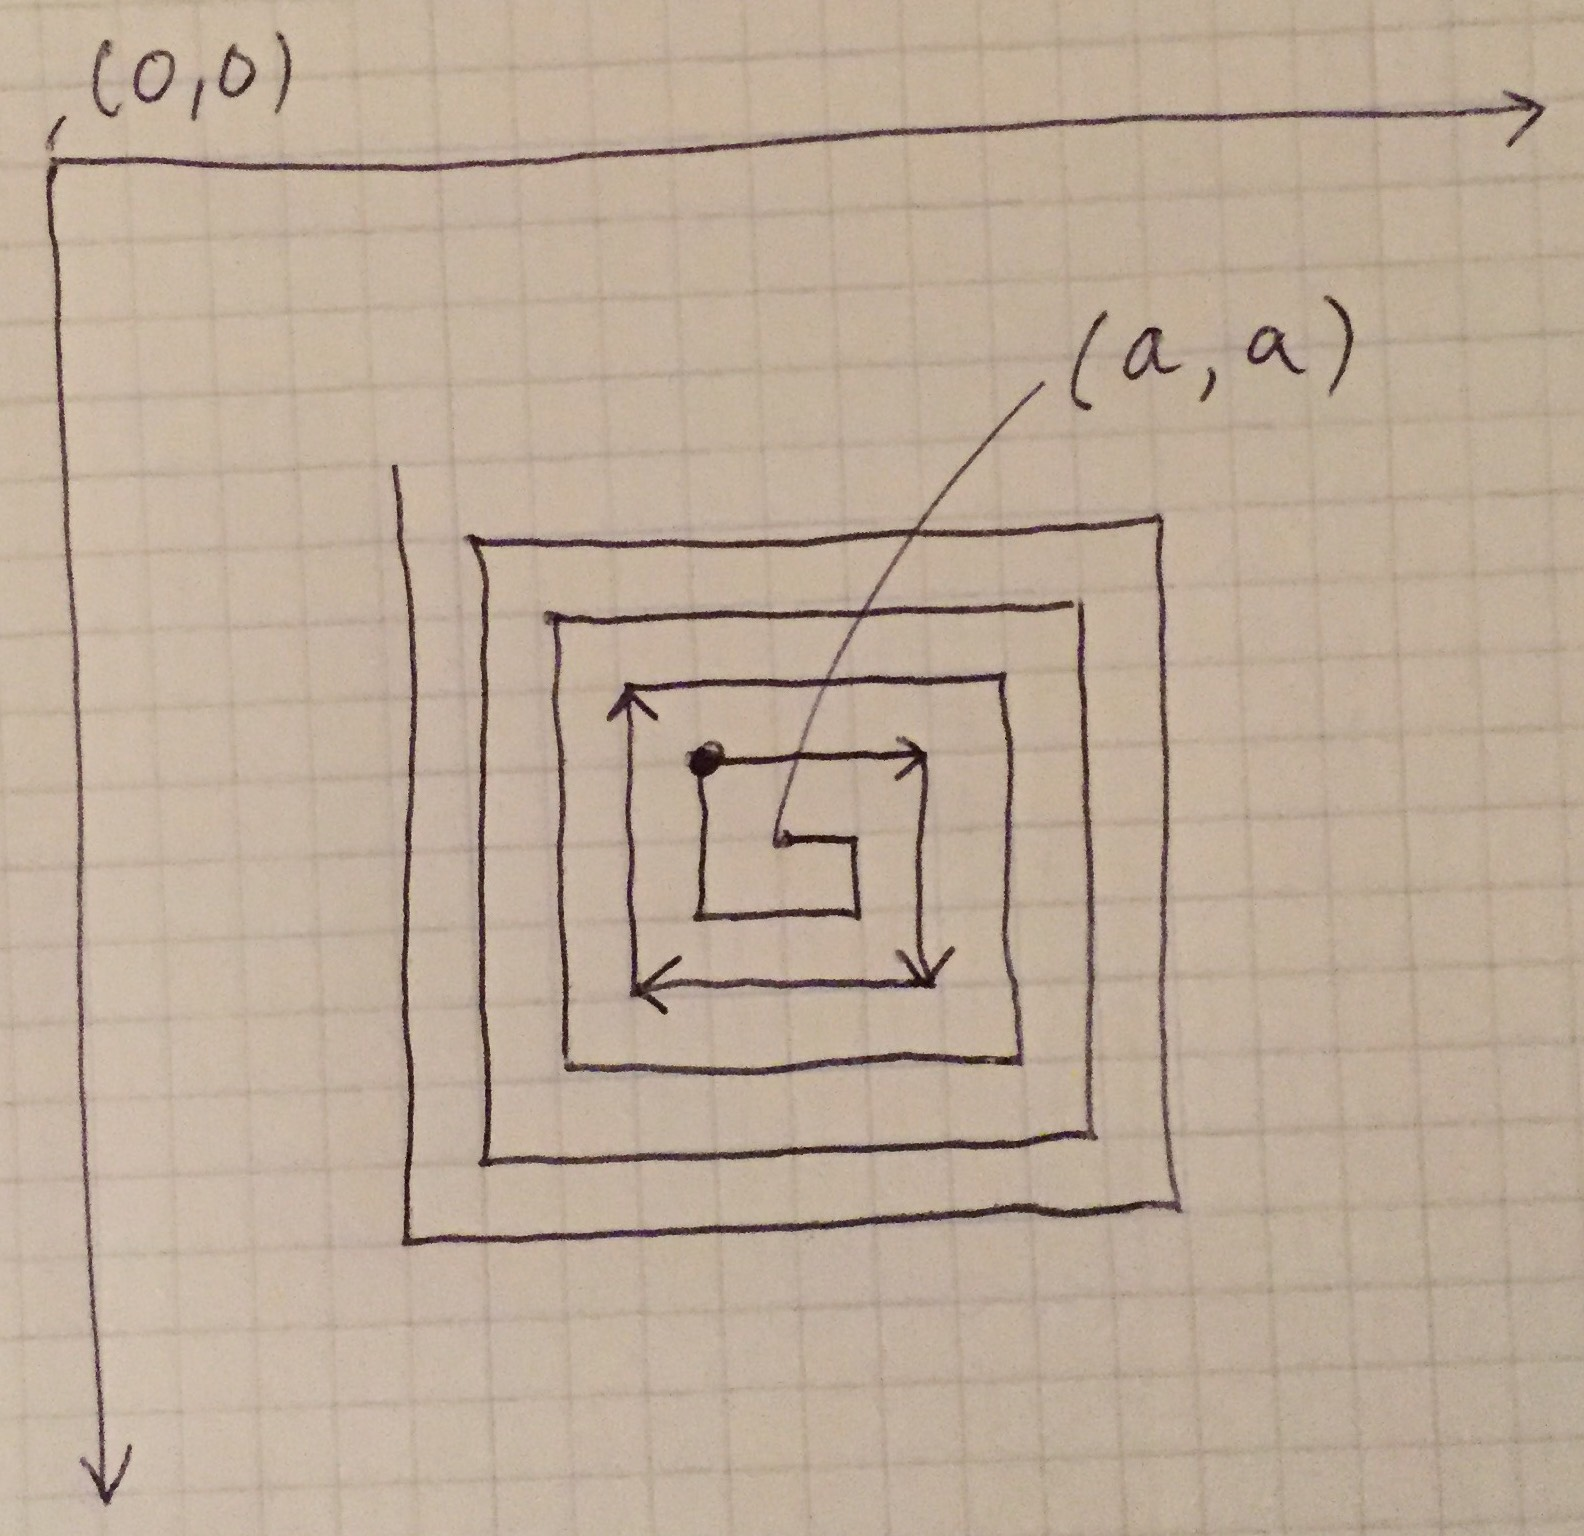
\includegraphics[height=0.75\textheight]{spiral.png}

\end{frame}

\end{document}
